\chapter{Anlagen} \label{Anlagen}
    \section*{Architektur}

    \begin{figure}[h]
        \centering
        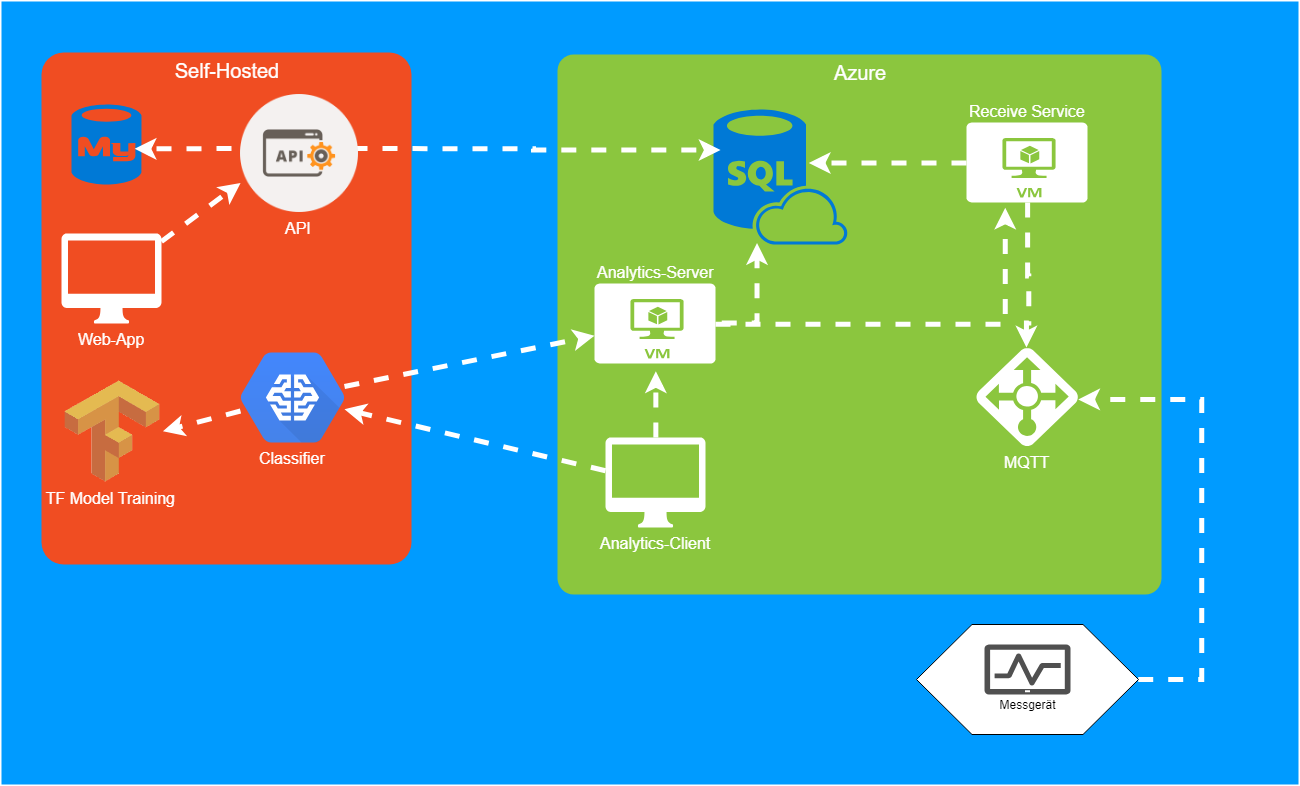
\includegraphics[width=1.0\textwidth]{ArchitectureComplete}
        \caption{Komplette Architektur \protect\cite{DrawIO}, \protect\cite{Tensorflow}}
        \label{fig:Architecture}
    \end{figure}

    \section*{Ergebnisse}

        \begin{figure}[H]
            \centering
            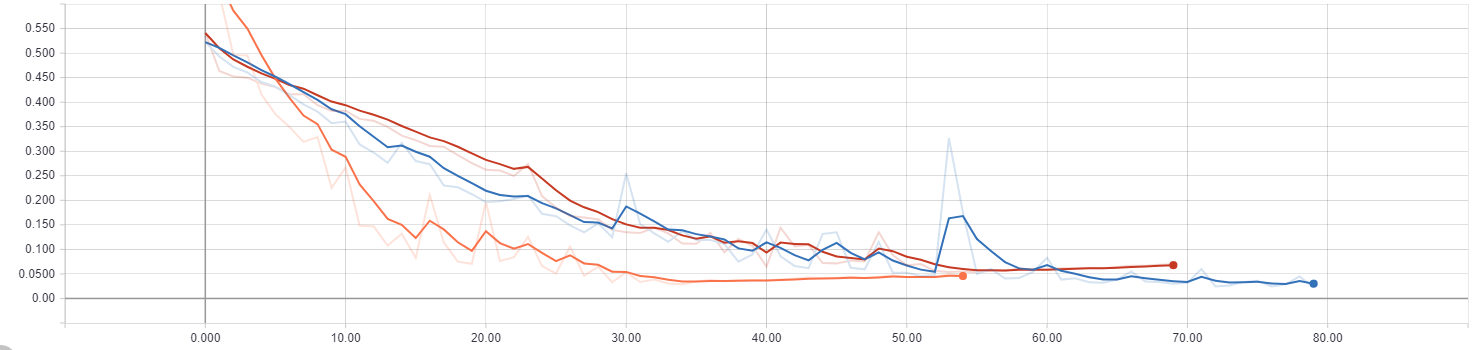
\includegraphics[width=1.0\textwidth]{val_loss_tensorboard_graph}
            \caption[Validation Loss von CNN, RNN and MIXED]{Validation Loss des Trainigs von CNN (blau), RNN (rot) und MIXED(orange) \protect\cite{Tensorflow}}
            \label{fig:ValLoss}
        \end{figure}

    \subsubsection{Epochen}

        Lernrate = 0.001\\
        \noindent
        Datentypen = ['u', 'h3', 'h5', 'h7', 'h9', 'h11', 'h13', 'h15']\\
        \noindent
        Batchgröße = 20\\

        \begin{table}[H]
            \centering
            \begin{tabular}{|c|c|c|c|}
                \hline
                Model & Epochen & Genauigkeit & Validierungsgenauigkeit \\
                \hline
                CNN & 10 &  87,38\% & 87,36\%  \\ 
                \hline
                RNN & 10 &  82,01\% & 81,22\%  \\ 
                \hline
                MIX & 10 &  83,28\% & 82,76\% \\ 
                \hline
                \hline
                CNN & 20 &  93,93\% & 92,09\%  \\ 
                \hline
                RNN & 20 &  84,41\% & 84,00\% \\ 
                \hline
                MIX & 20 &  86,68\% & 86,15\%  \\ 
                \hline
                \hline
                CNN & 30 &  96,75\% & 95,72\%  \\ 
                \hline
                RNN & 30 &  84,88\% & 84,57\%  \\ 
                \hline
                MIX & 30 &  88,23\% & 87,87\%  \\ 
                \hline
                \hline
                CNN & 40 &  98,18\% & 96,76\% \\ 
                \hline
                RNN & 40 &  85,18\% & 84,46\%  \\ 
                \hline
                MIX & 40 &  90,90\% & 89,72\%  \\ 
                \hline
                \hline
                CNN & 50 &  98,86\% & 97,50\%  \\ 
                \hline
                RNN & 50 &  85,80\% & 84,80\%  \\ 
                \hline
                MIX & 50 &  91,93\% & 91,10\%  \\ 
                \hline
                \hline
                CNN & 60 &  99,15\% & 98,58\%  \\ 
                \hline
                RNN & 60 &  85,67\% & 85,66\%  \\ 
                \hline
                MIX & 60 &  94,09\% & 90,53\%  \\ 
                \hline
                \hline
                CNN & 70 &  99,39\% & 99,02\%  \\ 
                \hline
                RNN & 70 &  86,63\% & 86,09\%  \\ 
                \hline
                MIX & 70 &  94,52\% & 92,94\%  \\ 
                \hline
                \hline
                CNN & 80 &  99,57\% & 99,27\%  \\ 
                \hline
                RNN & 80 &  86,22\% & 86,81\%  \\ 
                \hline
                MIX & 80 &  95,56\% & 93,98\%  \\ 
                \hline
                \hline
                CNN & 90 &  99,89\% & 99,63\%  \\ 
                \hline
                RNN & 90 &  87,64\% & 86,67\%  \\ 
                \hline
                MIX & 90 &  95,96\% & 94,42\%  \\ 
                \hline
                \hline
                CNN & 100 & 99,49\% & 99,37\%  \\ 
                \hline
                RNN & 100 & 87,29\% & 86,43\%  \\ 
                \hline
                MIX & 100 & 97,39\% & 96,46\% \\
                \hline

            \end{tabular}
            \caption[Ergebnis: komplette Epochen]{Ergebnis: komplette Epochen}
            \label{tabl:ErgebnisEpochComplete}
        \end{table}

        \section{API-Spezifikation}\label{API-Spezifikation}
        \subsubsection{Single Batch}
        \paragraph{Input:}

            \begin{lstlisting}[language=json,firstnumber=1]
Topic: "single-batch"
{
    "data": [
        {
            "u": float,
            "f": float,
            "h3": float,
            "h5": float,
            "h7": float,
            "h9": float,
            "h11": float,
            "h13": float,
            "h15": float,
        },
        .. x Batchsize
    ]
}
            \end{lstlisting}
        
            \paragraph{Output:}
        
            \begin{lstlisting}[language=json,firstnumber=1]
Topic: 'single-prediction'
{
    "data": float //- Prediction of Senseo
}
            \end{lstlisting}
    
        \subsubsection{Period}
            \paragraph{Input:}
    
                \begin{lstlisting}[language=json,firstnumber=1]
Topic: "period"
{
    "data": {
        "start": "DateTime2",
        "end": "DateTime2"
    }
}
                \end{lstlisting}
            
                \paragraph{Output:}
            
                \begin{lstlisting}[language=json,firstnumber=1]
Topic: 'period-prediction'
* Series of Predictions where 0: Senseo, 1: Microwave, 2: Bosch, 3: Undefined, for every second
{
    "data": [
        Int,
        ... end - start
        Int
    ]
}
                \end{lstlisting}
